\section{Appendix}

Here we provide additional evaluation results and details regarding
our implementations.

\subsection{Packet size}

{\sword} is designed to run at line rate, and is unperturbed by packet
size. In the case of Clover, its retries incur a significant bandwidth
overhead which causes additional slowdown when payloads are large.
Figure~\ref{fig:packet_size}, shows how {\sword} reacts to changes in
packet sizes. At 128 bytes the limitation is the load applied by
clients. At 256 bytes and above the 100-Gbps limit of the ConnectX-5
NICs becomes the bottleneck for read and write steering, and the
throughput drops proportionally.  Clover retries on larger packets are
more expensive than on smaller packets because the retry consumes
additional bandwidth on an already saturated link.

\begin{figure}
  \centering
  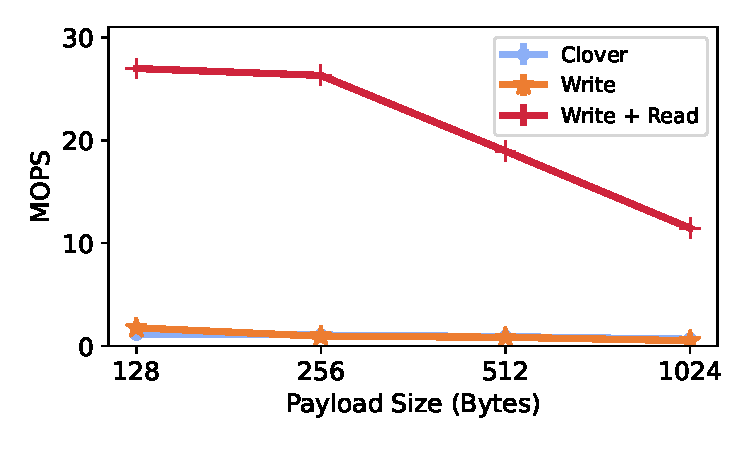
\includegraphics[width=0.485\textwidth]{fig/packet_size.pdf}

    \caption{Performance across RDMA payload sizes using 400 client cores at a
    50:50 read/write ratio.}

    \label{fig:packet_size}
\end{figure}

\subsection{Contention}

{\sword} is designed to operate well under even extreme contention. We
generate workloads at different points across a Zipf distribution.
The community standard for Zipf is 0.99; at this ratio the most
frequently requested key is requested around 17\% of the time. We
measure further down the distribution up to Zipf of 1.5, at which
point the hottest key is requested over 50\% of the time, and the
second hottest is around 20\%.  Figure~\ref{fig:contention} shows that
in the face of high contention 1.0 and above write and read steering
yields a 40$\times$ and above performance improvement at a 50\% write
workload. The decrease in read and write performance at high
contention is due to Clover's block allocator which becomes a
bottleneck with very hot keys.
%when keys are requests more than 30\% of the time.

\begin{figure}
  \centering
  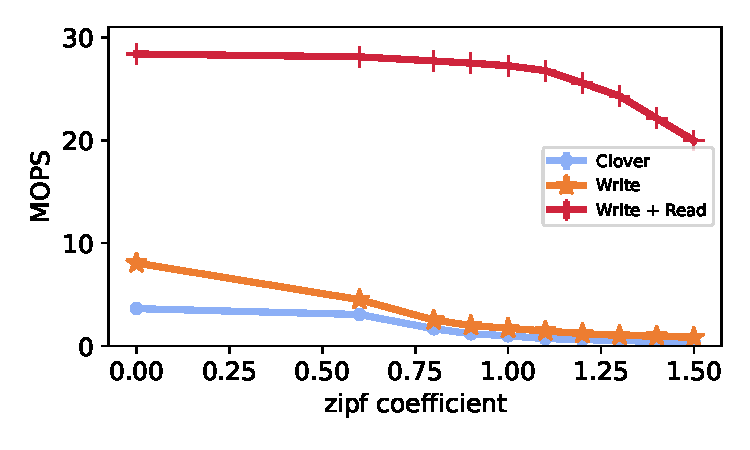
\includegraphics[width=0.485\textwidth]{fig/contention.pdf}

    \caption{Performance as contention increases with zipf coefficient using 400
    client cores on a 50\% write workload}

    \label{fig:contention}
\end{figure}

\subsection{Switch resources}
\label{sec:appendix_resources}

Figure~\ref{fig:switch_resources} provides a breakdown of the resource
consumption of our P4 \sword\ implementation. We collected these
values from our testbed using the barefoot SDE version 9.7.0. Each
reported percentage is the average value across the total 16 switch
pipeline stages. {\sword} fits into 8 stages, and is run entirely on
the ingress pipeline.

%\textbf{Switch Resource Utilization}
\begin{figure}[t]
    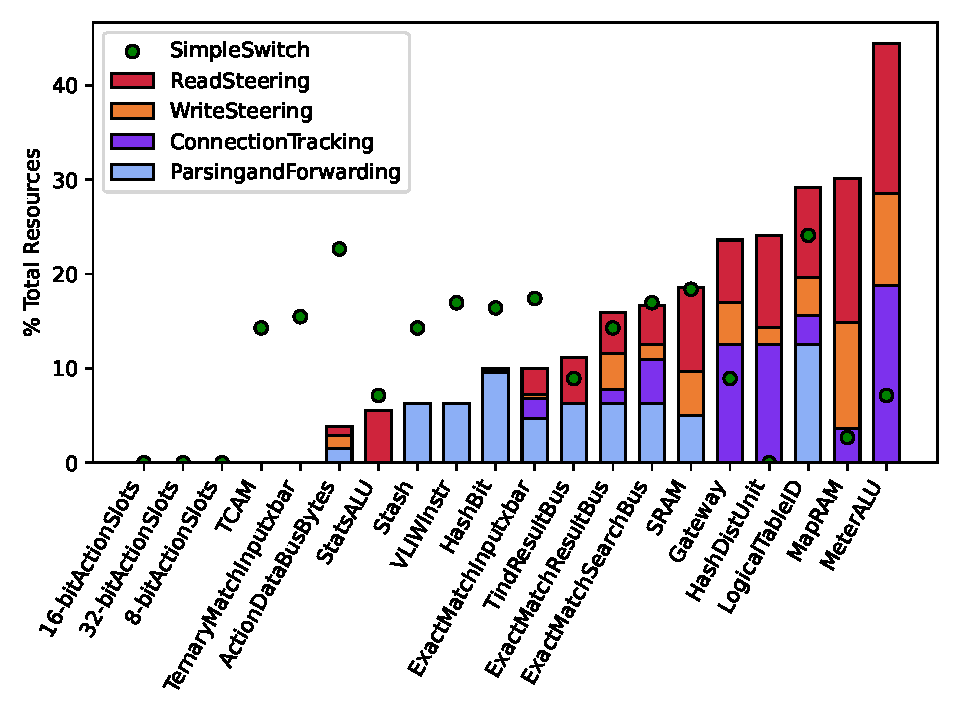
\includegraphics[width=0.485\textwidth]{fig/switch_resources.pdf}
%  \vskip -0.5em
    \caption{Breakdown of switch resource utilization by \sword\ component.}
    \label{fig:switch_resources}
%      \vskip -0.5em
\end{figure}



\subsection{RDMA ICRC}
\label{sec:appendix_icrc}

RDMA requests are not intended to be modified in flight, and care must
be taken not to corrupt them. RDMA invariant CRCs (ICRC) are
calculated at the time of sending and are designed to ensure the
integrity of the payload. When we modify requests their ICRC must be
recalculated or the packet will be rejected by the receiving NIC. Such
an error would cause an extreme performance hit as any dropped packet
triggers a timeout, and go-back-$n$ retransmission.  FPGA
implementations of RDMA ICRC have been built in the
past~\cite{Mansour_2019}; the required CRC calculation is identical to
Ethernet CRC, with some additional \texttt{crc32} for the
calculation. This algorithm is highly optimized for general case CRC
calcuation.

Recalculating the CRC for modified requests is the primary overhead of
{\sword} as it must be recalculated after a squence number update,
which occurs on all multiplexed and demultiplexed requests. This
overhead could be reduced by either removing the need for the CRC
(which is not a feature available on CX series NICs) or by allowing an
alterative, lightweight checksum which could be quickly updated based
on changes made to the packet while in flight. While these options are
not currently available we believe that commodity switches and
SmartNICs could leverage hardware offloads to reduce the cost, as the
CRC calculation is identical to Ethernet except masking
RoCE-specified packet felids.

%% We implemented RDMA ICRC in our DPDK prototype. To our knowledge no P4 switches
%% have native RoCEv2 support, while some projects have demonstrated that it is
%% possible to implement by hand, it requires many switch resources and adds
%% complexity~\cite{p4-telem} we forgot the additional complexity and turned off
%% ICRC checking on our CX5 NICs similar to prior work~\cite{switchml}. In the
%% future we hope that RoCEv2 checksums, like TCP, UDP,and Ethernet checksums can
%% be made hardware primitives on programmable switches.

\subsection{CXL} 
\label{sec:cxl}

CXL is a CPU-to-Device interconnect layered on PCIe 5.0 designed to
provide a coherent interface to devices, accelerators and
memory~\cite{cxl-spec}.  Although at the time of writing CXL is not a
commercially available technology, research prototypes have have
reported remote memory access latencies between
200-426ns~\cite{direct-cxl,microsoft-cxl-first-gen,facebook-cxl-tpp}.

CXL removes the DIMM slot constraint on per server memory capacity and provides
a way forward for high capacity memory pooling between many CPUs. The CXL
protocols do not provide opportunities for reducing or removing contention to
shared memory.  CLX.cache for instance exposes MESI states to the host CPU, and
levees coordination to them. This interface suggests that CXL devices will
suffer from identical lock contention problems as traditional memory with
inflated costs for coordination. Given that PCIe root complexes lack
programmability our techniques will likely not be applicable to CXL. We leave
resolving CXL memory contention to future work.
